%%%%%%%%%%%%%%%%%%%%%%%%%%%%%%%%%%%%%%%%%
% Stylish Article
% LaTeX Template
% Version 2.1 (1/10/15)
%
% This template has been downloaded from:
% http://www.LaTeXTemplates.com
%
% Original author:
% Mathias Legrand (legrand.mathias@gmail.com) 
% With extensive modifications by:
% Vel (vel@latextemplates.com)
%
% License:
% CC BY-NC-SA 3.0 (http://creativecommons.org/licenses/by-nc-sa/3.0/)
%
%%%%%%%%%%%%%%%%%%%%%%%%%%%%%%%%%%%%%%%%%

%----------------------------------------------------------------------------------------
%	PACKAGES AND OTHER DOCUMENT CONFIGURATIONS
%----------------------------------------------------------------------------------------

\documentclass[fleqn,10pt]{SelfArx} % Document font size and equations flushed left

\usepackage[english]{babel} % Specify a different language here - english by default

\usepackage{lipsum} % Required to insert dummy text. To be removed otherwise

\usepackage{subcaption} % Display multiple figures side by side

%----------------------------------------------------------------------------------------
%	COLUMNS
%----------------------------------------------------------------------------------------

\setlength{\columnsep}{0.55cm} % Distance between the two columns of text
\setlength{\fboxrule}{0.75pt} % Width of the border around the abstract

%----------------------------------------------------------------------------------------
%	COLORS
%----------------------------------------------------------------------------------------

\definecolor{color1}{RGB}{0,0,90} % Color of the article title and sections
\definecolor{color2}{RGB}{0,20,20} % Color of the boxes behind the abstract and headings

%----------------------------------------------------------------------------------------
%	HYPERLINKS
%----------------------------------------------------------------------------------------

\usepackage{hyperref}
\usepackage[T1]{fontenc} % Required for hyperlinks
\hypersetup{hidelinks,colorlinks,breaklinks=true,urlcolor=color2,citecolor=color1,linkcolor=color1,bookmarksopen=false,pdftitle={Title},pdfauthor={Author}}

%----------------------------------------------------------------------------------------
%	ARTICLE INFORMATION
%----------------------------------------------------------------------------------------

\JournalInfo{Kernel-Based Learning and Multivariate Modelling} % Journal information
\Archive{Fall 2019} % Additional notes (e.g. copyright, DOI, review/research article)

\PaperTitle{Understanding media-supported childhood education} % Article title

\Authors{Mikołaj Małkiński\textsuperscript{1}\textsuperscript{2}*} % Authors
\affiliation{\textsuperscript{1}\textit{Faculty of Mathematics and Information Science, Warsaw University of Technology, Warsaw, Poland}} % Author affiliation
\affiliation{\textsuperscript{2}\textit{Faculty of Computer Science of Barcelona, Universitat Politècnica de Catalunya, Barcelona, Spain}} % Author affiliation
\affiliation{*Email: malkinskim@student.mini.pw.edu.pl / mikolaj.malkinski@est.fib.upc.edu} % Corresponding author

\Keywords{Childhood education --- Data analysis --- Classification --- SVM --- XGBoost} % Keywords - if you don't want any simply remove all the text between the curly brackets
\newcommand{\keywordname}{Keywords} % Defines the keywords heading name

%----------------------------------------------------------------------------------------
%	ABSTRACT
%----------------------------------------------------------------------------------------

\Abstract{
Education during childhood can be highly beneficial for persons development.
Thanks to current state of technology it is possible to boost this process by supporting it with media devices.
This work tackles a challenge proposed in the \textit{2019 Data Science Bowl} competition which aims to understand key factors standing behind the learning process of young children.
Firstly, it performs an analysis of gameplay data gathered by a game-based learning application for children.
Then, it formulates a baseline model, constructs hand-crafted features based on domain knowledge and compares the results of different state-of-the-art models such as Support Vector Machines and XGBoost on the extended dataset.
Finally it discusses obtained results and presents further research directions which could improve the process of media-supported education for children.
}

%----------------------------------------------------------------------------------------

\begin{document}

\flushbottom % Makes all text pages the same height

\maketitle % Print the title and abstract box

\tableofcontents % Print the contents section

\thispagestyle{empty} % Removes page numbering from the first page

%----------------------------------------------------------------------------------------
%	ARTICLE CONTENTS
%----------------------------------------------------------------------------------------

\section{Introduction}

With recent advances in technology humans are presented with more and more opportunities to gain insights into the surrounding world.
Ability to gather tremendous amounts of data, high processing power of modern machines and possibilities for collaboration between researchers from different parts of the world make it possible to tackle challenging problems on a global scale.
Data Science Bowl is a platform created exactly for this purpose.
It organises competitions which focus on social good by gathering rich datasets and encourages researchers to collaborate on the solution.
Previous events were hosted on the Kaggle platform and tried to tackle problems such as heart disease detection~\cite{data-science-bowl-heart-diesase}, lung cancer detection~\cite{data-science-bowl-lung-cancer} or nuclei detection~\cite{data-science-bowl-nuclei},~\cite{Caicedo2019}.
This year, Data Science Bowl introduced a competition which main goal is to analyse how media can support learning outcomes in early childhood education~\cite{data-science-bowl-children}.

The data required for this challenge was collected with \textit{PBS KIDS Measure Up!} application, which is a game-based learning tool developed as a part of the \textit{CPB-PBS Ready to Learn} initiative, supported by the U.S. Department of Education.
It consists of anonymous gameplay data about played games and videos watched by children.
Based on this data, the goal is to predict how children will perform in their assessments.

This work will perform analysis on available dataset which will outline key characteristics of used education methods and propose ways for improvement.
Additionally, it will tackle the main challenge of predicting assessment scores by evaluating the performance of Support Vector Machines~\cite{svm} and comparing the results with other state-of-the-art methods.

%------------------------------------------------

\section{Dataset}

The dataset contains information about game analytics gathered by the \textit{PBS KIDS Measure Up!} application.
It places players into a fictional world where they can participate in different activities, games, video clips or assessments.
The Figure~\ref{fig:event-type-counts} presents the popularity of each part of the gameplay.
Each assessment is created with the goal of testing player's comprehension of a certain group of measurement-related skills.
They are divided into following categories: \textit{Bird Measurer}, \textit{Cart Balancer}, \textit{Cauldron Filler}, \textit{Chest Sorter}, and \textit{Mushroom Sorter}.

The goal of the competition is to predict the number of attempts a child will need to pass given assessment, based on the already gathered gameplay data.
Each incorrect answer is counted as an attempt.
The dataset is divided into two parts: training and testing.
The former one contains full history of gameplay data.
On the other hand, the latter one is missing history after starts of randomly chosen assessments, for which the number of attempts has to be predicted.
Furthermore, the outcomes of assessments are grouped into 4 categories: solved on the first attempt; solved on the second attempt; solved after 3 or more attempts; never solved.
Figures~\ref{fig:event-type-counts} and~\ref{fig:activity-time} give further insights into the dataset.

\begin{figure}
    \centering
    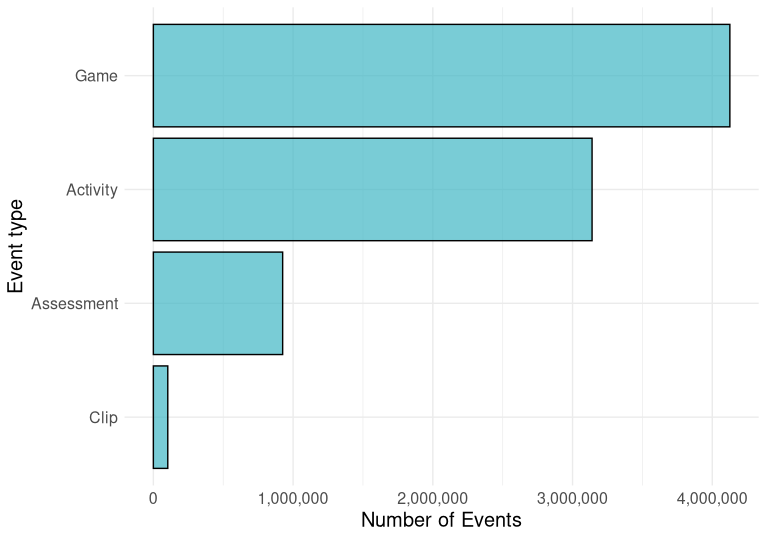
\includegraphics[width=\linewidth,height=6cm]{images/event-type-count.png}
    \caption{Count of events with given type. Most of the gameplay consists of games and activities, around 12.5\% is devoted to assessments whereas video clips are the rarest category.}
    \label{fig:event-type-counts}
\end{figure}

\begin{figure}
    \centering
    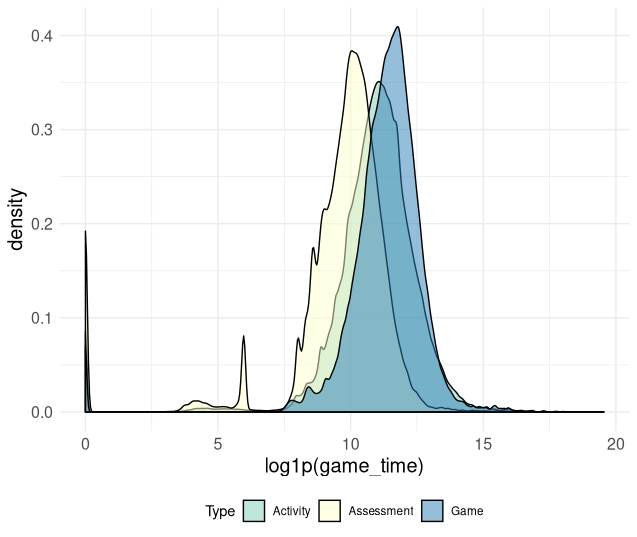
\includegraphics[width=\linewidth,height=6cm]{images/activity_time.png}
    \caption{Analysing the time spent on each gameplay category it's visible that most of the time is spent on games which are the most entertaining content in the application while least on assessments. Additionally there is a peak at the beginning which shows that some events are simply skipped by the user.}
    \label{fig:activity-time}
\end{figure}

%------------------------------------------------

\section{Methods}

This section will describe metrics, models and techniques such as data transformations used to improve the results.
Although the Kaggle platform gives the possibility to predict values for the test set and evaluate the performance, most of the experiments will either use cross-validation or a heldout validation set to assess the performance of the model.

\subsection{Evaluation metric}

To evaluate the submission, \textit{Quadratic Weighted Cohen's kappa coefficient} is used.
The general Cohen's kappa coefficient is defined as:
\begin{equation}
    \kappa = \frac{p_o - p_e}{1 - p_e}
    \label{eq:kappa}
\end{equation}
, where $p_o$ is the relative observed agreement among raters (accuracy) and $p_e$ is the hypothetical probability of chance agreement, using the observed data to calculate the probabilities of each observer randomly seeing each category.
In other words, $\kappa$ is a more robust metric than accuracy which takes into account the possibility of correct solutions occurring by chance.

\begin{table}[!h]
    \caption{Coefficients of a linear weighted $\kappa$ for a 4-class classification problem.}
    \centering
    \begin{tabular}{c|cccc}
        Class & 0 & 1 & 2 & 3 \\
        \hline
        0 & 0.00 & 0.33 & 0.67 & 1.00 \\
        1 & 0.33 & 0.00 & 0.33 & 0.67 \\
        2 & 0.67 & 0.33 & 0.00 & 0.33 \\
        3 & 1.00 & 0.67 & 0.33 & 0.00 \\
    \end{tabular}
    \label{tab:linear-kappa}
\end{table}

\begin{table}[!h]
    \caption{Coefficients of a quadratic weighted $\kappa$ for a 4-class classification problem.}
    \centering
    \begin{tabular}{c|cccc}
        Class & 0 & 1 & 2 & 3 \\
        \hline
        0 & 0.00 & 0.56 & 0.89 & 1.00 \\
        1 & 0.56 & 0.00 & 0.56 & 0.89 \\
        2 & 0.89 & 0.56 & 0.00 & 0.56 \\
        3 & 1.00 & 0.89 & 0.56 & 0.00 \\
    \end{tabular}
    \label{tab:quadratic-kappa}
\end{table}

The weighted $\kappa$ allows to weight disagreements differently - the score depends on the distance between predicted and actual class.
Recall that the considered challenge is a 4-class classification problem.
Table~\ref{tab:linear-kappa} presents weights used in a linear weighted $\kappa$.
They can also be thought as \textit{disagreement scores} - the larger the weight the higher disagreement between predicted and actual class.
To understand, consider the case when model predicts accuracy group 2 - the assessment was solved on the second attempt.
Then, if the prediction is correct the disagreement score is equal to $0$, if assessment was solved on the first attempt (class 3) or after 3 or more attempts (class 1) the prediction is off only by $1$ class and the disagreement score is $0.33$ and finally if it was never solved it equals to $0.67$.

The quadratic version allows to specify that the disagreement score depends not only on the difference between predicted classes but also on the order of the actual class.
The details of weights used in this case are shown in the Table~\ref{tab:quadratic-kappa}.

\subsection{Baseline model}

Firstly a naive model is created based on raw data to give a point of comparison for more advanced methods.
As the Figure~\ref{fig:assessment-accuracy-by-type} shows, there is a clear difference between assessment completion rates depending on the problem type.
The \textit{Chest Sorter} appears to be the hardest one having around 60\% of the attempts never solved, whereas \textit{Mushroom Sorter}, \textit{Cauldren Filler} and \textit{Cart Balancer} are usually solved after the first attempt.
Based on this observation a baseline model is built which is based on the median of accuracy groups - for a given child and type of assessment to predict, a median of all previous assessments of this child with given type is taken and this gives the predicted accuracy group.
This model achieved value of quadratic weighted $\kappa$ equal to $0.396$.

\begin{figure}
    \centering
    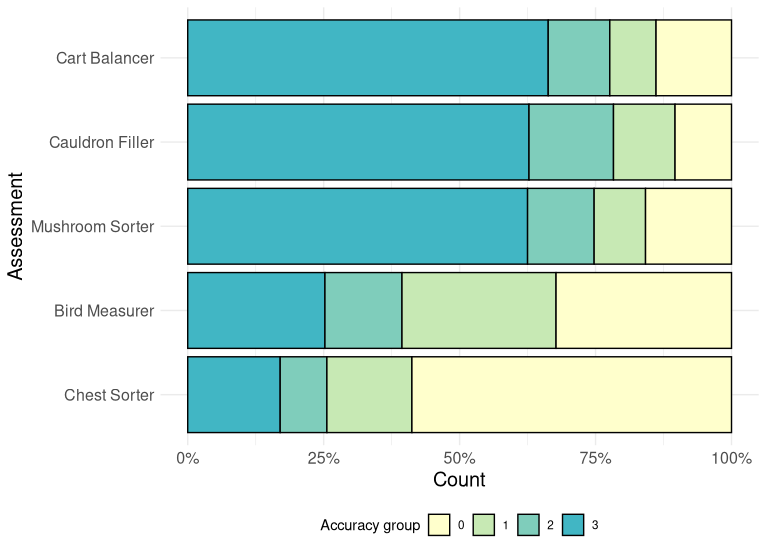
\includegraphics[width=\linewidth]{images/assessment-accuracy-group-count.png}
    \caption{Accuracy groups presented for each assessment type - the main idea behind the baseline model.}
    \label{fig:assessment-accuracy-by-type}
\end{figure}

\subsection{Feature engineering}

To potentially improve the performance of proposed models it may be beneficial to introduce hand-crafted features based on domain knowledge.
For this purpose the dataset was extended with fundamental summary statistics computed for each user.
The set of generated features contains the count of each activity in which user engaged, their accumulated and mean scores in each assessment, the number of successful and unsuccessful attempts, total counts of each event which occured during users gameplay history and some additional ones like the total or average time spent on each activity.
In total, the dataset was extended to more than 800 columns.
Furthermore, the original data contained more than 1 million records.
That is because each event which occurred during the gameplay was saved separately.
After described summarisation the new training set contains less than 18 thousand rows.
The same transformations were applied to the testing set.

With such large number of columns it is expected that some, if not most, of them will turn out to be useless.
In this case 2 approaches can be used: either one may try to analyse each feature separately by for example calculating its correlation with the response variable; or a feature selection method can be applied.
Without this procedure some classification models may have troubles in distinguishing which features are important and include them in the final prediction even though they are just random noise not correlated with the predicted feature.
What is more, the computation with such big dataset will take considerably more time than if the number of variables would be reduced.

\subsection{Feature selection}

\begin{figure}
    \centering
    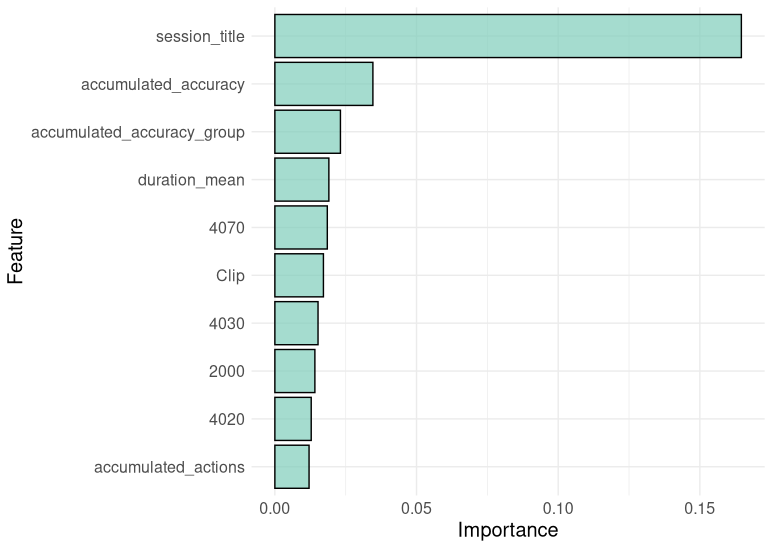
\includegraphics[width=\linewidth]{images/feature_importance.png}
    \caption{Feature ranking of XGBoost model with default parameters trained on the whole dataset for 10 most important variables.}
    \label{fig:feature-importance}
\end{figure}

To combat the \textit{curse of dimensionality} and reduce the dataset size a feature selection method has to be applied.
\paragraph{Iterative methods}
The first possibility is to use simple iterative methods like \textit{forward selection} which starts with a model without any features and then in each iteration adds a new variable; \textit{backward elimination} which starts with all features and then removes the least significant variable in each iteration; \textit{recursive feature elimination} which constantly creates new models while remembering the best and worst performing features at each iteration.
However, all described methods require a tremendous amount of iterations to find the best subset of predictors.
\paragraph{Ranking models}
Some of classification models are able to store additional information during training which tells about which feature was the most useful.
In this way it's possible to train a single model, such as XGBoost~\cite{xgboost}, and rank the variables by their importance.
Figure~\ref{fig:feature-importance} shows the 10 most important features selected by the XGBoost model from the whole set of more than 800 columns.
It's visible that a clear winner is the title of the assessment for which the accuracy group is predicted.
Other good variables are the accumulated accuracy and accuracy group for given player, as well as the average duration of the assessment - we can expect that users who solve a task in shorter time know the underlying reason standing behind the correct answer and don't require additional time for thinking.

\subsection{XGBoost}

\begin{figure}
    \centering
    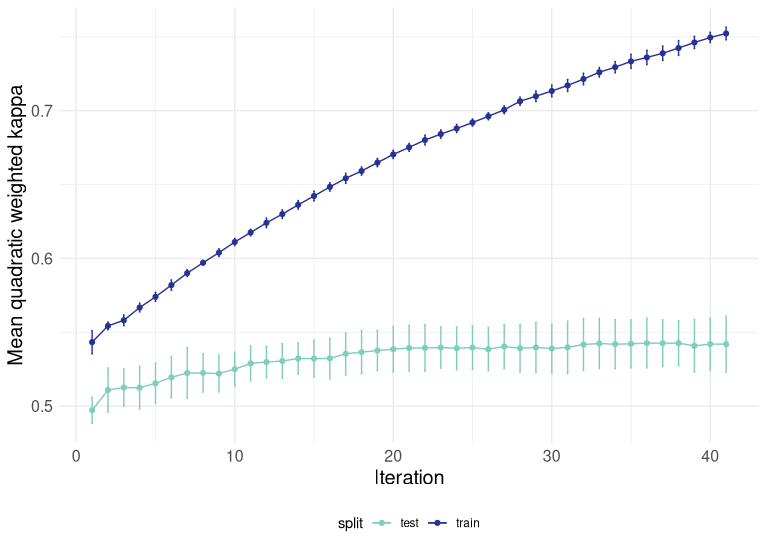
\includegraphics[width=\linewidth,height=6cm]{images/xgboost_cv.png}
    \caption{Value of mean quadratic weighted $\kappa$ with standard deviation averaged across 5 cross-validation folds for XGBoost.}
    \label{fig:xgboost-cv}
\end{figure}

Firstly the performance of state-of-the-art XGBoost model is analysed.
Figure~\ref{fig:xgboost-cv} shows the value of quadratic weighted $\kappa$ for the training and testing sets.
The results are averaged across 5 folds of cross-validation and \textit{early stopping} is used to stop the training if the metric doesn't improve on the testing set for more than 5 iterations.
It's clearly visible that the model overfits to the training data.
In order to improve the model performance and reduce overfitting, hyperparameter tuning is performed.
The complexity of an XGBoost model can be controlled by manipulating following parameters: \textit{max\_depth} controls the depth of generated trees - smaller trees have smaller predictive power but are less complex and have higher chance of generalising to the test set, bigger trees will more likely overfit to the train data; \textit{min\_child\_weight} which determines when to partition a leaf in the tree; \textit{subsample} which is the factor of training set to subsample for growing trees in each iteration; \textit{colsample\_bytree} determines the subsample ratio of features taken into consideration when building a new tree.

For each presented parameter a list of possible values was defined.
Then a method called \textit{random search} was performed which randomly sampled a value for each parameter and evaluated the model using 5-fold cross validation.
The best performing model achieved weighted quadratic $\kappa$ of $0.5411$ (averaged across 5 cross validation folds).

\subsection{Support Vector Machines}

\begin{figure}
    \centering
    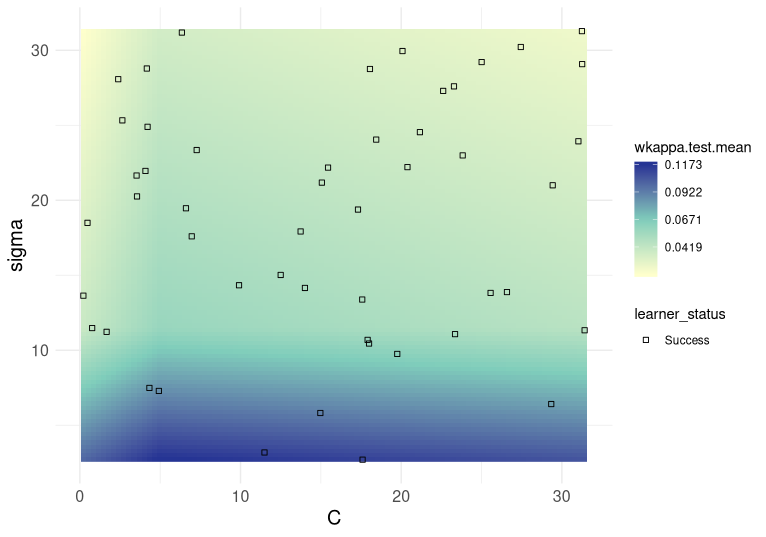
\includegraphics[width=\linewidth,height=6cm]{images/svm-optimisation.png}
    \caption{Heatmap showing 50 values of quadratic weighted $\kappa$ depending on randomly sampled parameters $C \in (2^{-5}, 2^5)$ and $\sigma \in (2^{-5}, 2^5)$ for SVM with rbfdot kernel, calculated on a heldout validation set.}
    \label{fig:svm-optimisation-1}
\end{figure}

Support Vector Machines (SVM) is another well performing model for classification tasks.
In presented experiments, the \textit{Radial Basis Function (RBF)} will be used as the kernel.
To achieve reasonable performance from an SVM it's necessary to carefully choose its parameters.
This work will analyse the influence of 2 parameters: $C$ - a regularisation parameter of the SVM, which is able to balance the trade-off between the amount of correctly classified observations from the training data and the margin of decision function;
$\sigma$ - inverse kernel width for the RBF kernel function.

For this purpose again the random search is applied.
Firstly, for a fixed kernel, different randomly sampled configurations of SVM's parameters $C \in (2^{-5}, 2^5)$ and $\sigma \in (2^{-5}, 2^5)$ are evaluated.
Figure~\ref{fig:svm-optimisation-1} presents a heatmap with values of quadratic weighted $\kappa$ depending on 50 randomly selected values of hyperparemeters.
The training time of an SVM, even with reduced number of features, is significantly larger compared to XGBoost.
Therefore for these experiments, cross validation was replaced with a heldout validation set, obtained by removing part of the training set.
Unfortunately, among all these configurations the highest performing one was able to achieve $\kappa = 0.1173$.
It's visible that higher values of $\kappa$ were achieved for lower values of $\sigma$, where it seems that $C$ doesn't make a big difference.
The random search procedure was repeated 2 more times with the same bounds for $C$, decreased bounds for $\sigma$ and 25 sampled configuraions in both cases.
Restricting $\sigma \in (2^{-8}, 2^3)$ allowed to find a solution with $\kappa = 0.2975$, whereas $\sigma \in (0, 1)$ allowed to find a solution with $\kappa = 0.3588$.

Obtained accuracies are reported on a heldout validation set - not whole training set was used for training.
Therefore a 5-fold cross validation was performed to achieve results comparable with XGBoost.
SVM achieved $\kappa = 0.3713$, which is surprisingly even lower than the baseline.

%------------------------------------------------

\section{Discussion}

\begin{table}
    \caption{Average quadratic weighted $\kappa$ of tested models.
    XGBoost turned out tu be the best performing model.
    Surprisingly, even after careful hyperparameter tuning, SVM wasn't able to beat the baseline.}
    \centering
    \begin{tabular}{c|c}
        Model & $\kappa$ \\
        \hline
        XGBoost & 0.5411 \\
        Baseline & 0.3713 \\
        SVM & 0.396 \\
    \end{tabular}
    \label{tab:model-results}
\end{table}

This work focused on analysing the possibilities of supporting childhood education with technology, by predicting childs performance in measurement based assessments.
Analysis and visualisation of the Data Science Bowl 2019 dataset give interesting insights into the way children interact with modern technological devices.
However, such a dataset requires in-depth knowledge about the considered domain in order to prepare hand-crafted features which can then be used by a learning model.
Most likely the features created in this work can still be improved by experts which could further boost the performance of evaluated models.
Moreover, to gain more insights into the problem, a wider selection of models should be evaluated on this dataset, starting from simple ones like logistic regression.
Further research should be conducted which could compare their performance to the heavy artillery used in this work - XGBoost and SVM.

Then, the performance of 2 state-of-the-art models was compared with a simple baseline.
XGBoost even with default parameter setting is able to achieve a significantly higher performance than constructed baseline.
On the other hand, SVMs achieved worse performance while requiring careful parameter tuning, processing time and computing resources.
The final achieved results are summarised in the Table~\ref{tab:model-results}.
However, it's important to remember that the SVM was trained only on 50 selected features from the dataset, which were chosen as the most crucial by XGBoost.
It might turn out that other variables are more important for good performance of SVM, which were not included in this set.
Nonetheless, exploring this possibility would require a significantly larger computing possibilities even to train the model with default parameters, but then what about cross-validation and hyperparameter tuning?

%----------------------------------------------------------------------------------------
%	REFERENCE LIST
%----------------------------------------------------------------------------------------
\phantomsection
\bibliographystyle{unsrt}
\bibliography{report}

%----------------------------------------------------------------------------------------

\end{document}
